\chapter{Data}

Because there is intrinsic variability in the number of near-Earth objects colliding with Earth's atmosphere from night to night, a sufficiently large data sample plays a vital role in estimating an average flux.
This chapter details our data sample.
Specifically we will discuss into observable time, observable area, and number of events.  
To assess the overall capabilities of our system, we also delve into the data behind our star catalog, previously used for total observable area calculations.  
This chapter provides the raw data and overall distribution and shape of the data. Further analysis and interpretation of the data can be found in Chapter 5.

\section{Time Distributions}

While the D6 AllSky Camera has a protective watertight shell, it is currently not always placed outside for nightly observations due to precaution and convenience.
Due to Oregon's climate, we often leave our observation system inside.
There have been a total of $221$ days between August 27, 2018, the beginning of Willamette's academic year, and May 6, 2019.
Out of those $221$ days, we have observed during $34$ nights, for a total of $291.87$ hours.

When outside, the D6 AllSky Camera automatically begins observation runs when the sky is dark enough to take videos of without fear of over-saturation.
As the sky gets brighter when sunrise approaches, the camera automatically shuts off, ending the observation session.
This brightness constraint means that the total observation time changes from night to night.
During observation nights, we observed for an average of $8.584$ hours per night.
The shortest observation session lasted $7$ hours while the longest lasted $11$ hours.

Figure~\ref{dateplot} displays the individual nights that we observed throughout the academic calendar. 
In addition to plotting our observation dates and each session's total observing time, we have indicated dates of meteor showers visible in Salem, Oregon.  
During the months of October and November, we observed on nights of the Orionid and Leonid showers respectively.  
% Insert smooth transition

\begin{figure}[ht!]
  \centering
  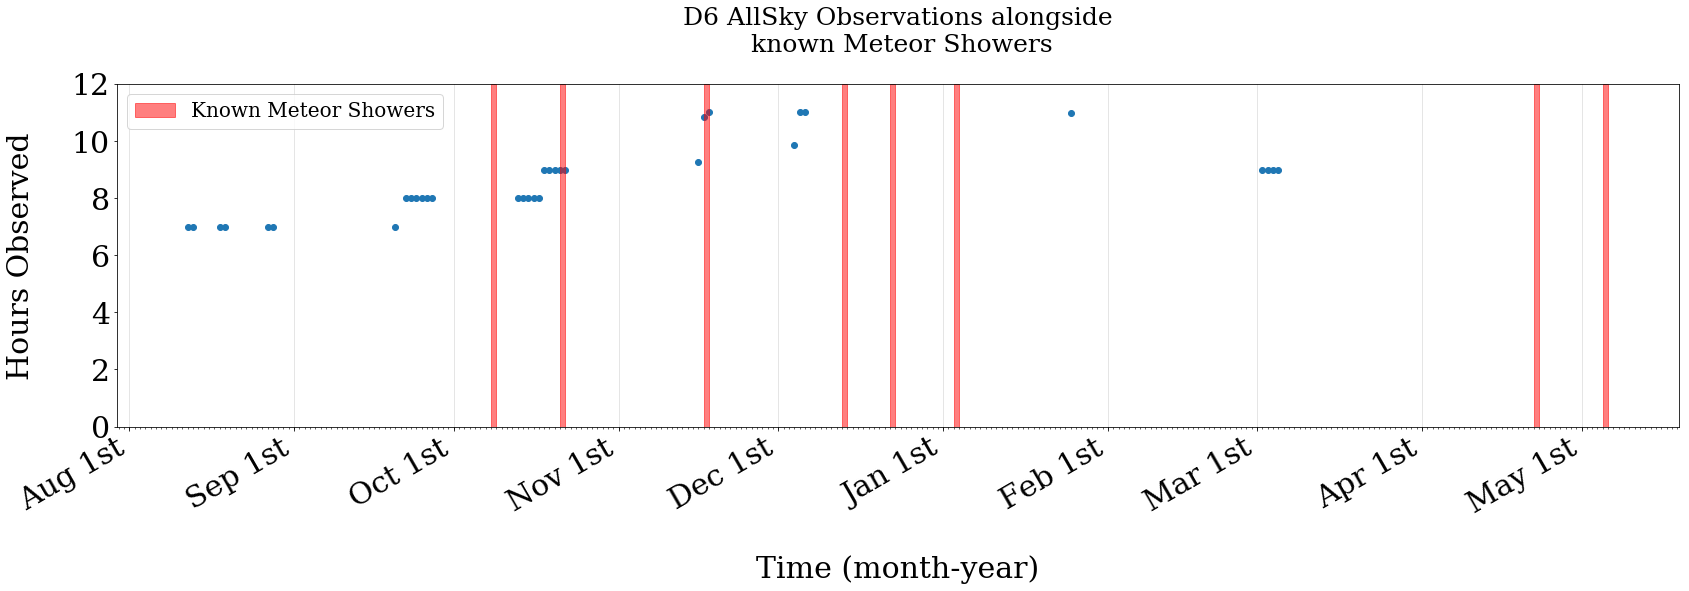
\includegraphics[scale=0.25]{images/nights_observed_with_meteorshowers.png}
  \caption[A plot of all D6 AllSky observation dates and recognized meteor showers within the $2018-2019$ academic calendar year.]{A plot of all D6 AllSky observation dates and recognized meteor showers within the $2018-2019$ academic calendar year.  Note significant time gaps between observations as well as crossover between observations and meteor showers.}
  \label{dateplot}
\end{figure}




\section{Coverage Distributions}

As described in the methodology section, to calculate the angular distance per pixel for a given location, we needed two celestial object measurements.
These measurements can represent data from the same objects, but the two must have different pixel locations.
By taking the angular separation between the two, we designated the ratio to be at the midpoint between both locations.  
In total, we used $3279$ different comparisons to compile our angular distance per pixel dataset.  
Figure~\ref{angperpix1} shows all of these points, each colored with their respective angular separation per pixel ratio. 
We observe that some data points seem to follow natural arcs.
This is a result of to same-celestial object comparisons as they arc through the night's sky over time.


\begin{figure}[ht!]
  \centering
  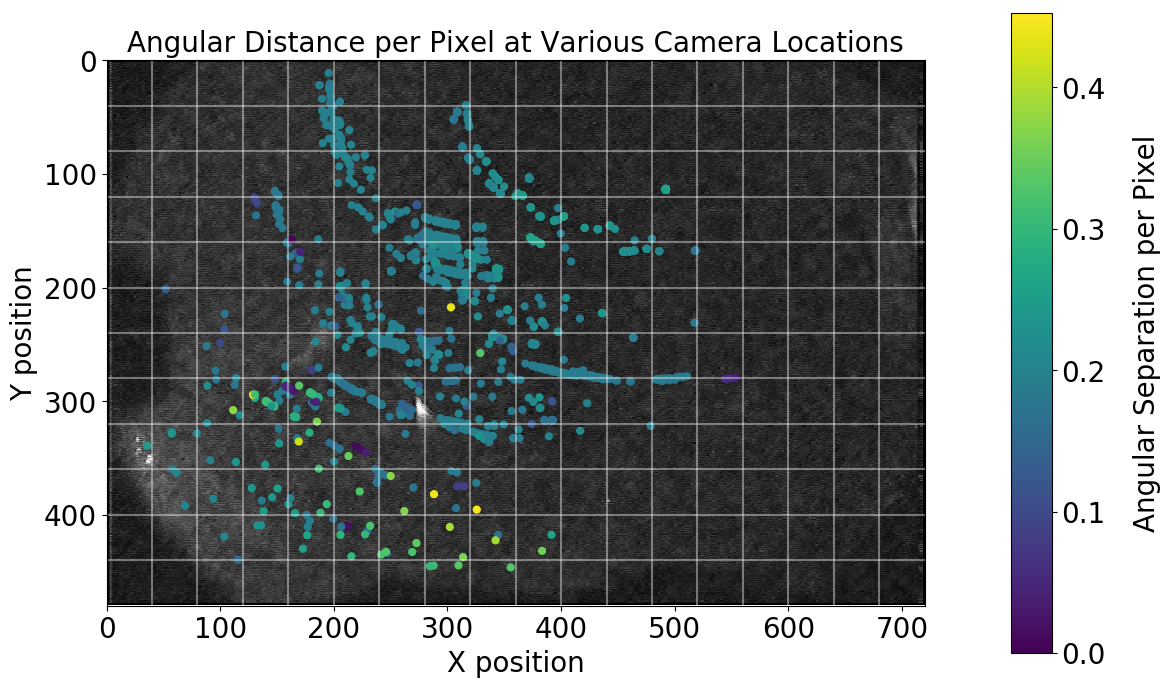
\includegraphics[scale=0.47]{images/angular_distance_at_various_locations.png}
  \caption[A plot of initial angular distance per pixel measurements from celestial comparisons before rotation.]{A plot of initial angular distance per pixel measurements from celestial comparisons before rotation.  Here we see that a radial symmetry argument is necessary to get data points in bins that are not covered.  The arc-like patter in the data is representative of the path of a celestial object through the night's sky.}
  \label{angperpix1}
\end{figure}

One may note that Figure~\ref{angperpix1} shows many data points, but they do not span the entirety of the camera field. 
By rotating our initial data and appending it to a larger data set in sequences of $5\degree$ in a full unit circle, we were able to increase the number of data points by a magnitude of $71.22$ and cover all pixel regions in our field of view.
From this point we were able to then bin the data and create Fig~\ref{colorful}.
We bin and average the data to get an overall idea of how pixel distances relate to angular distances in different smaller regions.
Fig~\ref{colorful} shows how these average relationships vary in different regions of our field of view, as indicated by their color value.

\begin{figure}[ht!]
  \centering
  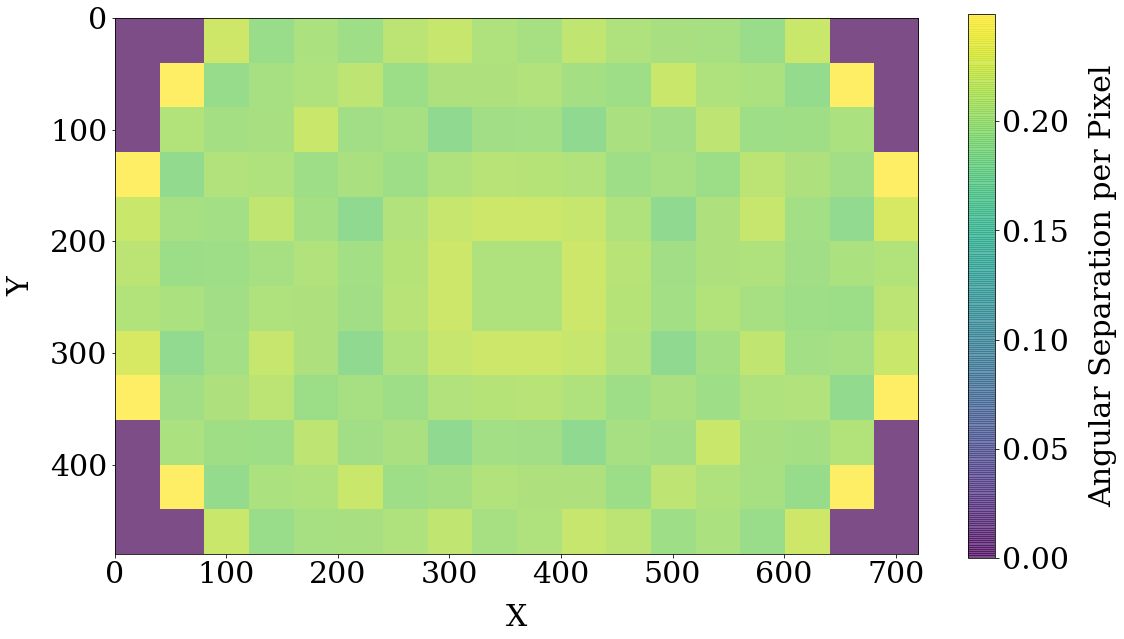
\includegraphics[scale=0.35]{images/boxes_colored.png}
  \caption[Average angular separation per pixel for different camera pixel regions.]{Average angular separation per pixel for different camera pixel regions.  We observe a larger angular separation per pixel closer to the horizon.  This aligns well with our prediction of the fish-eye camera's effect. Note the color bar reads differently than the previous image.}
  \label{colorful}
\end{figure}

As described in the Background chapter, we used our measured solid angles for each region to calculate individual  curved-rectangular areas at a fixed radius of \SI{11.4}{\kilo\meter}.
Our measured total areal coverage was  \SI{48363.33}{\square\kilo\meter}.

As some nights were cloudy and others clear, the observable area fluctuated from night to night. 
Figure~\ref{time_area} summarizes the total observation time and the average observable area for each of our observation months. 

\begin{figure}[ht!]
  \centering
  \makebox[\textwidth][c]{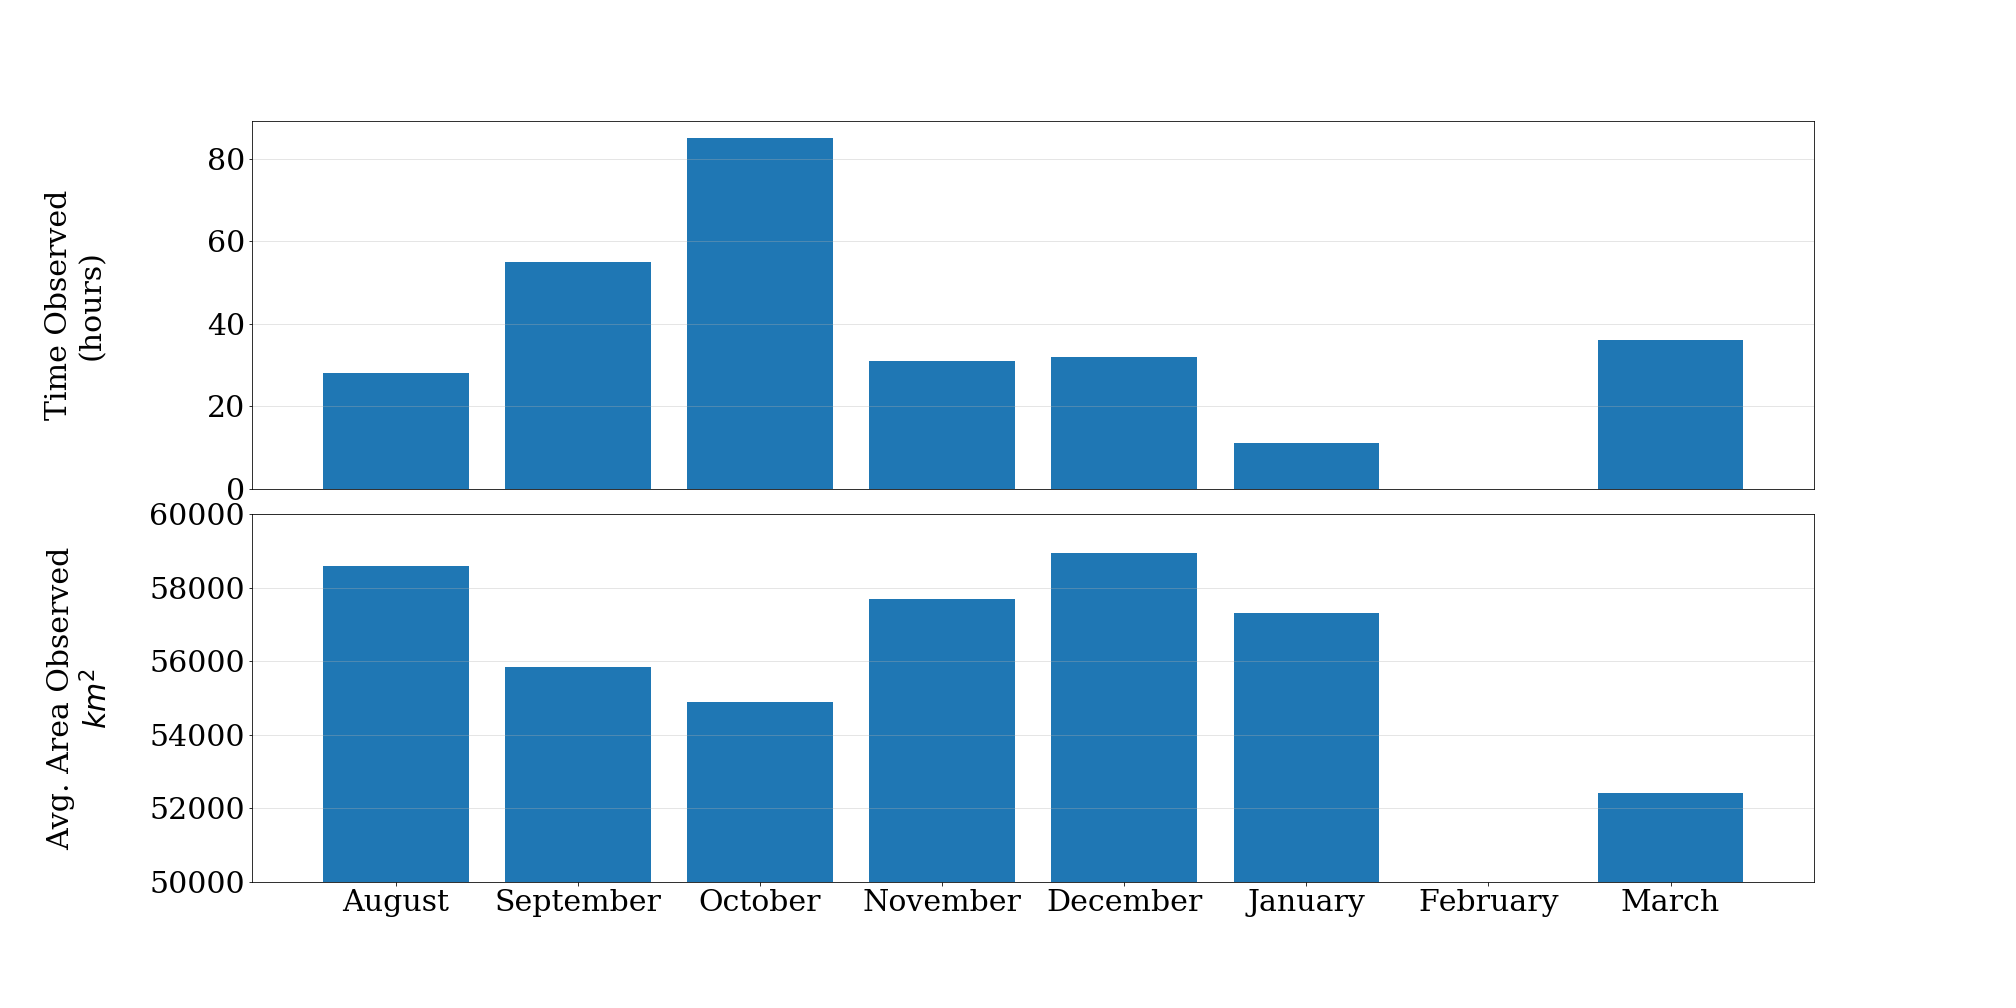
\includegraphics[width=1.2\textwidth]{images/time_vs_areaobs_plot.png}}
  \caption[A plot of total observation time and average observable area for each month.]{A plot of total observation time and average observable area for each month.  Note that in October we observed for the longest and under the worst observable area conditions.  This is likely a result of the two meteor showers that occur during that month.  We see a dip in time observed as we approach winter/early spring months, as expected.}
  \label{time_area}
\end{figure}

Our average observable area across all observations was  \SI{46178.81}{\square\kilo\meter}.
This value, along with our total observation time and number of events was used to determine the overall average flux.

\section{Detected Fireballs}

In total, the D6 AllSky Camera captured a total of $1077$ videos.  
Of those $1077$, only $6$ were identified as real fireballs.
Most of these false positives were caused by fast moving clouds or bugs.
In November, we began running a newly implemented secondary analysis that was created by Jed Rembold.
This analysis greatly reduces the number of false positives.
In the three months prior to the implementation of this analysis, there were $793$ videos from $3$ months of data.
Post-implementation, we captured $284$ videos in the remaining $4$ months containing observations.
A depiction of the locations of our captured fireballs is shown in Figure~\ref{fireball_locs}.
While the data sample is still small, we can observe that the locations of these fireballs are not dependent on a specific region of our field of view.  

\begin{figure}[ht!]
  \centering
  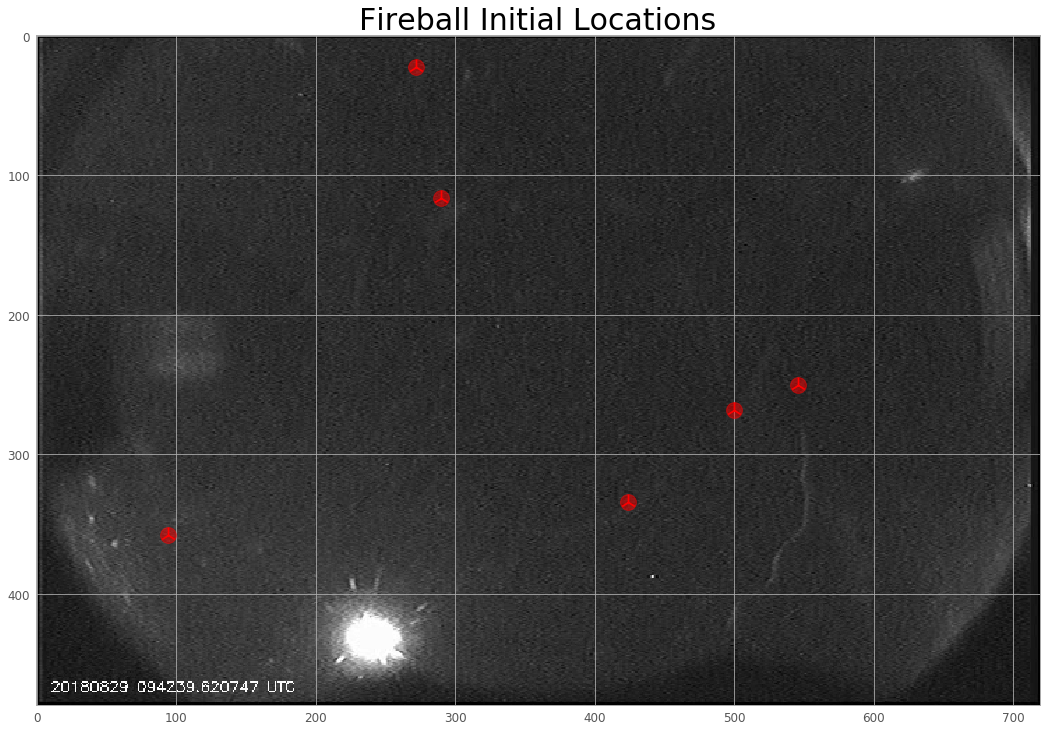
\includegraphics[scale=0.25]{images/fireball_initlocs.png}
  \caption[The initial pixel locations of all detected fireballs with respect to our field of view.]{The initial pixel locations of all detected fireballs with respect to our field of view.  Note that the locations are not dependent or specific to any region in our field of view.}
  \label{fireball_locs}
\end{figure}

Of the $6$ fireballs, $3$ were found within $24$ hours of the Leonid meteor shower while $1$ more was found during the Orionid meteor shower.  

Unfortunately, the photometry program used to analyze fireball light-curves had issues processing each of these cases, and there was not enough time to troubleshoot and fix that program.  
Therefore, we do not have calibrated luminosities for our observed fireballs and can not make a prediction of their energy or mass at the moment. 


\section{Camera Capabilities}

As described in Chapter 3, the star catalog consists of recognized stars from the D6 AllSky Camera's snapshots.
In a catalog containing a total of $387$ celestial object observations we observed an average of $1.44$ stars per snapshot containing at least one star.
In total, the system took $1638$ snapshots or videos that could be condensed to snapshots via frame-stacking.
$269$ of these contained identifiable celestial objects (stars or the moon).  
Within our star catalog, we captured information on $14$ unique objects.
Of these objects, the dimmest, Alpheratz, had a visible apparent magnitude of $2$. 
Sirius was our brightest recognized star, having a magnitude of $-1.46$.
It should be noted that the moon, having an apparent magnitude of $-12.74$, is significantly brighter than any observable star apart from the sun.


\section{Flux}

After attaining the number of events, total observation time, and average observational area, we found that the D6 AllSky Camera had an average flux of \SI{4.45E-7}{\per\hour\per\square\kilo\meter}.
Table~\ref{table1} displays this value alongside the values that contributed to our flux calculation. 
As a point of comparison, Dr.~Jed Rembold measured an average flux rate of \SI{1.09E-7}{\per\hour\per\square\kilo\meter} when studying meteor impacts on the Moon \cite{jed_dissertation_2014}. 
Clearly the Moon and Earth are inherently two different objects with different gravitational effects.
However they have similar locations within our solar system, and thus their average flux rates should share some resemblance.
The fact that the D6 AllSky Camera's fireball flux rate shares the same order of magnitude as other meteor research is promising.  
While we can't make any definitive claims about the feasibility of our camera system, we remain cautiously optimistic. 



\begin{table}[ht]
\setlength\extrarowheight{5pt}
\centering
\begin{tabular}{lll}
\toprule
& D6 AllSky Camera & Lunar Impacts \\
\midrule
Number of Events & $6$ & $51$  \\
%\hline
Average Area (km$^2$) & $46,178.81$ & $5.77 \times 10^{6}$ \\
%\hline
Total Time (hr) & $291.87$ & $80.97$ \\
\midrule
Flux (hr$^{-1}$km$^{-2}$) & $4.45 \times 10^{-7}$ & $(1.09 \pm 0.02) \times 10^{-7}$ \\
\bottomrule
%\hline
\end{tabular}
\caption[A display of our average flux rate alongside contributing variables compared to lunar impact flux rates measured by Dr. Jed Rembold \cite{jed_dissertation_2014}.]{A display of our average flux rate alongside contributing variables compared to lunar impact flux rates measured by Dr. Jed Rembold \cite{jed_dissertation_2014}. Note that while the many of the contributing variables are significantly different, both flux measurements are on the same order of magnitude.}
\label{table1}
\end{table}

